\documentclass[10pt,a4paper]{article}
\usepackage[slovak]{babel}
\usepackage[utf8]{inputenc}
\usepackage{amsmath}
\usepackage{amsfonts}
\usepackage{amssymb}
\usepackage[unicode]{hyperref}
\usepackage{graphicx}

\textwidth 6.5in
\oddsidemargin 0.0in
\evensidemargin 0.0in

\title{Poznámky z Úvodu do databázových systémov - materiál na štátnice}
\date{16.06.2012}
\author{Peter Csiba, petherz@gmail.com, \url{https://github.com/Petrzlen/fmfi-poznamky}} 

\begin{document}
\maketitle
\tableofcontents

\clearpage

%%%%%%%%%%%%%%%%%%%%%%%%%%%%%%%%%%%%%%%%%%%%%%%%%%%%%%%%%%%%%%%%%%%%%%%%%%%%%%%%
%%%%%%%%%%%%%%%%%%%%%%%%%%%%%%%%%%%%%%%%%%%%%%%%%%%%%%%%%%%%%%%%%%%%%%%%%%%%%%%%
\section*{Úvod}   

Text je poznámkami k oficiálnym \href{http://new.dcs.fmph.uniba.sk/index.php/Studium/Bakalarske/StatneSkusky}{štátnicovým otázkam} a boli spísané počas učenia sa na ne.
Poznámky sa nesnažia ísť do hĺbky (na to je H.Garcia-Molina, Ullman a Wikipédia).
Naopak, snažia sa priniesť intuitívnu predstavu o algoritmoch a pojmoch a dávať ich do súvisu.

Poznámky sú organizované podľa štátnicových otázok, snažia sa minimalizovať omáčku a nevysvetlujú a neuvádzajú do problematiky. Text je určený čitateľom, ktorý sa už s hlavnými pojmami stretli.
Autor považuje všetky otázky za rovnako dôležité a odporúča v prípade slabšieho pochopenia samostatne vypracovať niektoré staré \href{http://www.dcs.fmph.uniba.sk/~plachetk/TEACHING/DB2011/index.html}{písomky}.

Autor absolvoval základný test predmetu Úvodu do databázových systémov s hodnotením A, a má základné skúsenosti s administráciou a návrhom databáz. Napriek tomu autor \underline{neručí za kvalitu a úplnosť textu} a čitateľov \underline{aj} preto autor \underline{prudko odporúča pozrieť si aj iné zdroje}. Uvedieme citát\footnote{Dr. Tomas Plachetka, Uvod do databazovych systemov 2011/2012 Zima} ''Tieto slajdy sú sprievodcom pri prednáške, nie sú myslené ako náhrada
prednášky či nebodaj knihy. K príprave na skúšku nestačí len prečítať slajdy'', niečo také sú aj tieto poznámky.  

Nakoniec poznamenajme, že autor sa snažil písať pravdu a len pravdu, keďže jeho odpoveď na záverečných skúškach vychádza z tototo materiálu.
Ak čitateľ chce prispieť ku kvalite textu, nech autorovi napíše a ten mu udelí prístup do repozitára.

P.S. Autor zistil, že názvoslovie pijan, ľúbi, krčma, alkohol použil už napríklad \href{http://csip.sk/uploads/ullman.pdf}{Ullman}.

%%%%%%%%%%%%%%%%%%%%%%%%%%%%%%%%%%%%%%%%%%%%%%%%%%%%%%%%%%%%%%%%%%%%%%%%%%%%%%%%
%%%%%%%%%%%%%%%%%%%%%%%%%%%%%%%%%%%%%%%%%%%%%%%%%%%%%%%%%%%%%%%%%%%%%%%%%%%%%%%%
\section*{Úvod a motivácia databáz}
\paragraph{Účel.}
\begin{itemize}
\item Zobrazenie vybranej časti reality v počítačí.
\item Uchovávanie informácií v konzistentnom stave a ich pridávanie.
\item Poskytovanie informácií (dotazy, reporty - periodické správy). 
\item Ochrana informácií pred zničením a neoprávneným prístupom. 
\end{itemize}

\paragraph{Charakteristiky DBMS (Database Management System).}
\begin{itemize}
\item Dáta majú štruktúru, ktorá sa zriedka mení, objem dát je veľký.
\item Dáta nie sú uložené na užívateľovom počítači, pre prístup k dátam sa využíva počítačová sieť (klient-server).
\item Dotazy sú zložité.
\item Množstvo užívateľov pristupuje k dátam súčasne.
\item Vyžaduje sa vysoká priepustnosť.
\item Vyžaduje sa vysoká odolnosť voči poruchám.
\item Vyžaduje sa vysoký stupeň bezpečnosti.
\item Prístup koncových užívateľov k dátam musí byť jednoduchý(API, GUI).
\end{itemize}

\paragraph{Porovnanie dotazov v dátových modeloch.}
Vo všeobecnosti sa snažíme zbaviť všeobecných kvatifikátorov pomocou pravidla $\forall P \rightarrow \not \exists \not P$.

Máme tabuľky: 
\begin{itemize}
\item studenti(Student, Skupina)
\item rozvrh\_skupiny(Skupina, Miestnost, Cas)
\item rozvrh\_ucitelia(Ucitel, Skupina)
\end{itemize}

\begin{itemize}
\item \emph{Hovorovo.} Treba nájsť (všetky) štvorice [Student, Miestnost, Cas, Ucitel]
také, že ten učiteľ učí toho študenta v tej miestnosti a tom čase. 
\item \emph{Predikátový kalkul.}

\{[Student, Miestnost, Cas, Ucitel]: $\exists$ Skupina (Student, Skupina) $\wedge$ rozvrh\_skupiny(Skupina, Miestnost, Cas) $\wedge$ rozvrh\_ucitelia(Ucitel, Skupina)\}
\item \emph{Relačná algebra.}
$$
\Pi_{student, miestnost, cas, ucitel}(studenti \Join rozvrh_skupiny \Join rozvrh_ucitelia)
$$
\item \emph{Datalog (Prolog).}
\begin{verbatim}
rozvrh_studenti(Student, Miestnost, Cas, Ucitel) <--
\begin{verbatim}
  studenti(Student, Skupina),
  rozvrh_skupiny(Skupina, Miestnost, Cas),
  rozvrh_ucitelia(Učitel, Skupina).

? rozvrh_studenti(S, M, C, U)
\end{verbatim} 

\item \emph{SQL.}
\begin{verbatim}
SELECT S.student, RK.miestnost, RK.cas, RU.ucitel
FROM studenti S, rozvrh_skupiny RK, rozvrh_ucitelia RU
WHERE S.skupina=RK.skupina AND S.skupina=RU.skupina
\end{verbatim}

\end{itemize}

%%%%%%%%%%%%%%%%%%%%%%%%%%%%%%%%%%%%%%%%%%%%%%%%%%%%%%%%%%%%%%%%%%%%%%%%%%%%%%%%
%%%%%%%%%%%%%%%%%%%%%%%%%%%%%%%%%%%%%%%%%%%%%%%%%%%%%%%%%%%%%%%%%%%%%%%%%%%%%%%%
%TODO vynechava stranu, (asi) lebo article a section* a section
\section{Dátové modely} 
\href{http://en.wikipedia.org/wiki/Database_model}{Pozri Wikipédiu.}

\paragraph{Používané dátové modely.}
\begin{itemize}
\item Entitno-relačný. Pozri \ref{entity_relationship}. 
\item Relačný. Pozri \ref{relacny_kalkul} a \ref{relacna_algebra}. 
\item Navigačný (XML). Stromová štruktúra, dotazovací jazyk XPath a XQuery. 
\item Objektový. Niečo ako objekty v programovaní. Objekty okrem zapuzdrenia dát špecifikujú prístup k nim a k ich vzťahom, je možné s nimi programaticky narábať. Napríklad DOM (Document Object Model). 
\end{itemize}


%%%%%%%%%%%%%%%%%%%%%%%%%%%%%%%%%%%%%%%
\subsection{Trojschémová architektúra (ANSI sparc)}

\paragraph{Úrovne.}
\begin{itemize}
\item Konceptuálna úroveň (všeobecná databázová schéma). 
\item Interná úroveň (špecifikácia polí, kľúčov, indexov, ...).
\item Fyzická úroveň. Algoritmy a dátové štruktúry, využtie diskového priestoru. Pozri \ref{fyzicka_organizacia}.
\end{itemize}

\begin{center}
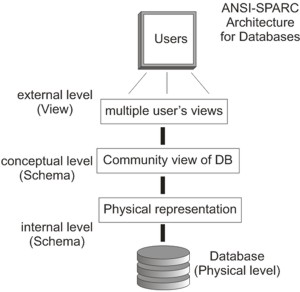
\includegraphics{db_ansi_sparc.jpg}
\end{center} 

\paragraph{Vlastnosti.}
\begin{itemize}
\item Nezávislý pohľad užívateľov. Každý môže použiť svoj dotazovací jazyk. 
\item Užívateľ nevidí fyzickú organizáciu dát. Tá sa môže zmeniť, bez toho, aby to užívateľ postrehol. 
\end{itemize}

%%%%%%%%%%%%%%%%%%%%%%%%%%%%%%%%%%%%%%%
\subsection{Entitno-relačný model}
\label{entity_relationship}

Máme entity (tabuľky, polia, ...) a vzťahy medzi nimi. 
\paragraph{Typy vzťahov.}
\begin{itemize}
\item One-to-one (1-1). Napríklad hlava a telo. 
\item One-to-many (1-n). Napríklad vozidlo a kolesá. 
\item Many-to-many (n-m). Napríklad kupujúci a produkt (táto dvojica nemusí byť unikátna).
\end{itemize}

\begin{center}
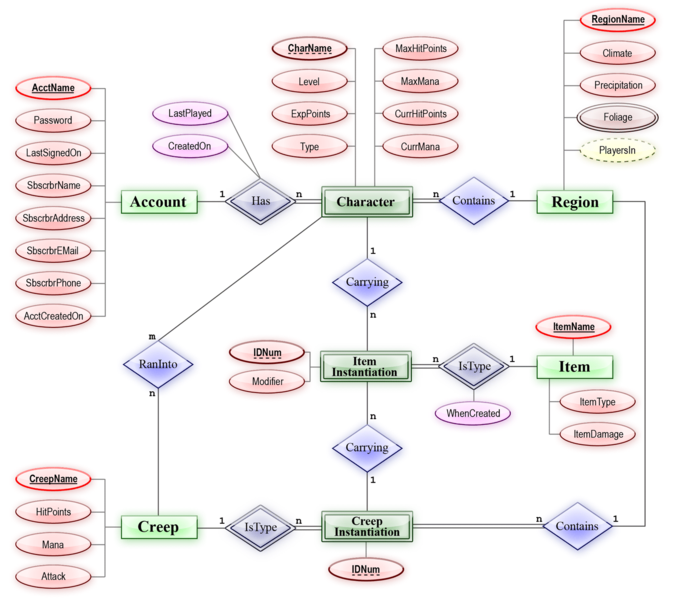
\includegraphics[scale=0.5]{db_entity_relationship.png}
\end{center} 

%%%%%%%%%%%%%%%%%%%%%%%%%%%%%%%%%%%%%%%
\subsection{Relačný model, relačná algebra}
Pozri \ref{relacny_kalkul} a \ref{relacna_algebra}. 

%%%%%%%%%%%%%%%%%%%%%%%%%%%%%%%%%%%%%%%
\subsection{Negácia a rekurzia v relačnej algebre}
Pozri \ref{relacna_algebra}. 

%%%%%%%%%%%%%%%%%%%%%%%%%%%%%%%%%%%%%%%
\subsection{Súvis relačnej algebry s inými dotazovacími jazykmi}
Pozri \ref{relacna_algebra_suvis}.
    
%%%%%%%%%%%%%%%%%%%%%%%%%%%%%%%%%%%%%%%%%%%%%%%%%%%%%%%%%%%%%%%%%%%%%%%%%%%%%%%%
%%%%%%%%%%%%%%%%%%%%%%%%%%%%%%%%%%%%%%%%%%%%%%%%%%%%%%%%%%%%%%%%%%%%%%%%%%%%%%%%
\section{Relačný kalkul} 
\label{relacny_kalkul}

Deklaruje výroky, ktoré ohraničujú výsledok dotazu. 

%%%%%%%%%%%%%%%%%%%%%%%%%%%%%%%%%%%%%%%
\subsection{Predikátová interpretácia relačnej algebry}


%%%%%%%%%%%%%%%%%%%%%%%%%%%%%%%%%%%%%%%
\subsection{Negácia, doménovo nezávislé a bezpečné formuly}
%%%%%%%%%%%%%%%%%%%%%%%%%%%%%%%%%%%%%%%
\subsection{Relačný kalkul (doménový)}
%%%%%%%%%%%%%%%%%%%%%%%%%%%%%%%%%%%%%%%
\subsection{Súvis relačného kalkulu s inými dotazovacími jazykmi}
    
%%%%%%%%%%%%%%%%%%%%%%%%%%%%%%%%%%%%%%%%%%%%%%%%%%%%%%%%%%%%%%%%%%%%%%%%%%%%%%%%
%%%%%%%%%%%%%%%%%%%%%%%%%%%%%%%%%%%%%%%%%%%%%%%%%%%%%%%%%%%%%%%%%%%%%%%%%%%%%%%%
\section{Datalog} 
%%%%%%%%%%%%%%%%%%%%%%%%%%%%%%%%%%%%%%%
\subsection{Syntax a sémantika Datalogových programov}
%%%%%%%%%%%%%%%%%%%%%%%%%%%%%%%%%%%%%%%
\subsection{Súvis s relačným kalkulom}
%%%%%%%%%%%%%%%%%%%%%%%%%%%%%%%%%%%%%%%
\subsection{Výpočet dotazu na Datalogový program}
%%%%%%%%%%%%%%%%%%%%%%%%%%%%%%%%%%%%%%%
\subsection{Negácia}
%%%%%%%%%%%%%%%%%%%%%%%%%%%%%%%%%%%%%%%
\subsection{Bezpečnosť Datalogových programov}
    
%%%%%%%%%%%%%%%%%%%%%%%%%%%%%%%%%%%%%%%%%%%%%%%%%%%%%%%%%%%%%%%%%%%%%%%%%%%%%%%%
%%%%%%%%%%%%%%%%%%%%%%%%%%%%%%%%%%%%%%%%%%%%%%%%%%%%%%%%%%%%%%%%%%%%%%%%%%%%%%%%
\section{Relačná algebra} 
\label{relacna_algebra}

%%%%%%%%%%%%%%%%%%%%%%%%%%%%%%%%%%%%%%%
\subsection{Operátory relačnej algebry}
%%%%%%%%%%%%%%%%%%%%%%%%%%%%%%%%%%%%%%%
\subsection{Multimnožinová interpretácia relácií}
%%%%%%%%%%%%%%%%%%%%%%%%%%%%%%%%%%%%%%%
\subsection{Grupovanie a agregácia}
%%%%%%%%%%%%%%%%%%%%%%%%%%%%%%%%%%%%%%%
\subsection{Rekurzia, výpočet pevného bodu}
%%%%%%%%%%%%%%%%%%%%%%%%%%%%%%%%%%%%%%%
\subsection{Súvis relačnej algebry s inými dotazovacími jazykmi}
\label{relacna_algebra_suvis}
    
%%%%%%%%%%%%%%%%%%%%%%%%%%%%%%%%%%%%%%%%%%%%%%%%%%%%%%%%%%%%%%%%%%%%%%%%%%%%%%%%
%%%%%%%%%%%%%%%%%%%%%%%%%%%%%%%%%%%%%%%%%%%%%%%%%%%%%%%%%%%%%%%%%%%%%%%%%%%%%%%%
\section{Jazyk SQL} 
%%%%%%%%%%%%%%%%%%%%%%%%%%%%%%%%%%%%%%%
\subsection{Programovanie v SQL (Data Definition Language, Data Manipulation Language)}
%%%%%%%%%%%%%%%%%%%%%%%%%%%%%%%%%%%%%%%
\subsection{Negácia a rekurzia v SQL}
%%%%%%%%%%%%%%%%%%%%%%%%%%%%%%%%%%%%%%%
\subsection{Súvis SQL s inými dotazovacími jazykmi}
    
%%%%%%%%%%%%%%%%%%%%%%%%%%%%%%%%%%%%%%%%%%%%%%%%%%%%%%%%%%%%%%%%%%%%%%%%%%%%%%%%
%%%%%%%%%%%%%%%%%%%%%%%%%%%%%%%%%%%%%%%%%%%%%%%%%%%%%%%%%%%%%%%%%%%%%%%%%%%%%%%%
\section{Teória navrhovania relačných báz dát} 

%%%%%%%%%%%%%%%%%%%%%%%%%%%%%%%%%%%%%%%
\subsection{Funkčné závislosti}
%%%%%%%%%%%%%%%%%%%%
\paragraph{Armstrongove axiómy.} 
%%%%%%%%%%%%%%%%%%%%
\paragraph{Uzáver množiny atribútov.}
%%%%%%%%%%%%%%%%%%%%
\paragraph{uzáver množiny funkčných závislostí.}

%%%%%%%%%%%%%%%%%%%%%%%%%%%%%%%%%%%%%%%
\subsection{Pokrytie a minimálne pokrytie množiny funkčných závislostí}
%%%%%%%%%%%%%%%%%%%%%%%%%%%%%%%%%%%%%%%
\subsection{Nadkľúče a kľúče}
    
%%%%%%%%%%%%%%%%%%%%%%%%%%%%%%%%%%%%%%%%%%%%%%%%%%%%%%%%%%%%%%%%%%%%%%%%%%%%%%%%
%%%%%%%%%%%%%%%%%%%%%%%%%%%%%%%%%%%%%%%%%%%%%%%%%%%%%%%%%%%%%%%%%%%%%%%%%%%%%%%%
\section{Normálne formy} 
%%%%%%%%%%%%%%%%%%%%%%%%%%%%%%%%%%%%%%%
\subsection{3NF, BCNF}
%%%%%%%%%%%%%%%%%%%%%%%%%%%%%%%%%%%%%%%
\subsection{Algoritmy pre dekompozíciu do normálnych foriem}
%%%%%%%%%%%%%%%%%%%%%%%%%%%%%%%%%%%%%%%
\subsection{Bezstratovosť dekompozície}
    
%%%%%%%%%%%%%%%%%%%%%%%%%%%%%%%%%%%%%%%%%%%%%%%%%%%%%%%%%%%%%%%%%%%%%%%%%%%%%%%%
%%%%%%%%%%%%%%%%%%%%%%%%%%%%%%%%%%%%%%%%%%%%%%%%%%%%%%%%%%%%%%%%%%%%%%%%%%%%%%%%
\section{Transakcie} 
%%%%%%%%%%%%%%%%%%%%%%%%%%%%%%%%%%%%%%%
\subsection{Požiadavky na transakčný systém (ACID)}
%%%%%%%%%%%%%%%%%%%%%%%%%%%%%%%%%%%%%%%
\subsection{Architektúra transakčného systému}
%%%%%%%%%%%%%%%%%%%%%%%%%%%%%%%%%%%%%%%
\subsection{Rozvrhy}
%%%%%%%%%%%%%%%%%%%%%%%%%%%%%%%%%%%%%%%
\subsection{Triedy sériovateľnosti a obnoviteľnosti}
    
%%%%%%%%%%%%%%%%%%%%%%%%%%%%%%%%%%%%%%%%%%%%%%%%%%%%%%%%%%%%%%%%%%%%%%%%%%%%%%%%
%%%%%%%%%%%%%%%%%%%%%%%%%%%%%%%%%%%%%%%%%%%%%%%%%%%%%%%%%%%%%%%%%%%%%%%%%%%%%%%%
\section{Implementácia sériovateľnosti a obnoviteľnosti v transakčných systémoch} 
%%%%%%%%%%%%%%%%%%%%%%%%%%%%%%%%%%%%%%%
\subsection{Testy sériovateľnosti}
%%%%%%%%%%%%%%%%%%%%%%%%%%%%%%%%%%%%%%%
\subsection{Algoritmy izolácie, zámky, časové pečiatky, validácia}
%%%%%%%%%%%%%%%%%%%%%%%%%%%%%%%%%%%%%%%
\subsection{Uviaznutie (deadlock) a metódy riešenia uviaznutia}
%%%%%%%%%%%%%%%%%%%%%%%%%%%%%%%%%%%%%%%
\subsection{Algoritmy obnovy, log-file, checkpointing, backup}
    
%%%%%%%%%%%%%%%%%%%%%%%%%%%%%%%%%%%%%%%%%%%%%%%%%%%%%%%%%%%%%%%%%%%%%%%%%%%%%%%%
%%%%%%%%%%%%%%%%%%%%%%%%%%%%%%%%%%%%%%%%%%%%%%%%%%%%%%%%%%%%%%%%%%%%%%%%%%%%%%%%
\section{Fyzická organizácia} 
\label{fyzicka_organizacia}

%%%%%%%%%%%%%%%%%%%%%%%%%%%%%%%%%%%%%%%
\subsection{Dvojúrovňový model pamäti a organizácie dát}
%%%%%%%%%%%%%%%%%%%%%%%%%%%%%%%%%%%%%%%
\subsection{Indexové stromy, hashovanie}
%%%%%%%%%%%%%%%%%%%%%%%%%%%%%%%%%%%%%%%
\subsection{Operátory fyzickej algebry}
%%%%%%%%%%%%%%%%%%%%%%%%%%%%%%%%%%%%%%%
\subsection{Implementácia vybraných fyzických operátorov (merge-sort, nested-loop join)}


%%%%%%%%%%%%%%%%%%%%%%%%%%%%%%%%%%%%%%%%%%%%%%%%%%%%%%%%%%%%%%%%%%%%%%%%%%%%%%%%
%%%%%%%%%%%%%%%%%%%%%%%%%%%%%%%%%%%%%%%%%%%%%%%%%%%%%%%%%%%%%%%%%%%%%%%%%%%%%%%%
\clearpage
\section*{Referencie a odporúčaná literatúra}
\begin{itemize}                                
\item \href{http://www.dcs.fmph.uniba.sk/~plachetk/TEACHING/DB2011/index.html}{Úvodu do databázových systémov - Plachetka}.        
\item \href{http://www.dcs.fmph.uniba.sk/~sturc/databazy/uvod/}{Úvodu do databázových systémov - Šturc} - v niečom detailnejší.        
\item \href{http://infolab.stanford.edu/~widom/cs145/}{Úvodu do databázových systémov - Stanford University} - základ podobný.


\item \href{http://csip.sk/uploads/plachetka\_uvod\_do\_databaz\_2011.pdf}{Plachetkove slide-i}.
\item \href{http://csip.sk/uploads/ullman.pdf}{Ullmanove slide-i}.
\item \href{http://fmfi-uk.hq.sk/Informatika/Uvod\%20Do\%20Databazovych\%20Systemov/prednasky/}{Mandos}.
\item H. Garcia-Molina, J.D. Ullman, J. Widom: Database Systems, The Complete Book, Prentice Hall, 2003
\item R. Elmasri, S.B. Navathe: Fundamentals of Database Systems, Addison-Wesley, 2006
\item Na poslednú otázku\footnote{
Na ktorej už zopár ľudí dostalo Fx.
}: S. Lightstone, T.J. Teorey, T. Nadeau: Physical Database Design, Morgan Kaufmann, 2007
\end{itemize}

\end{document}
